\documentclass[11pt]{article}

\usepackage[margin=1in]{geometry}
\usepackage[T1]{fontenc}
\usepackage[utf8]{inputenc}
\usepackage{lmodern}
\usepackage{amsmath}
\usepackage{amssymb}
\usepackage{booktabs}
\usepackage{hyperref}
\usepackage{enumitem}
\usepackage{array}
\usepackage{xcolor}
\usepackage{tikz}
\usepackage{pgfplots}
\usepackage{float}
\usepackage{caption}

\pgfplotsset{compat=1.18}
\usetikzlibrary{arrows.meta, positioning, shapes.geometric, fit, calc}

\hypersetup{
  colorlinks=true,
  linkcolor=blue,
  urlcolor=blue
}

\setlist[itemize]{noitemsep, topsep=4pt}
\setlist[enumerate]{noitemsep, topsep=4pt}
\setlength{\parskip}{0.45em}
\setlength{\parindent}{0pt}

\definecolor{global}{HTML}{7A4F9A}
\definecolor{transition}{HTML}{C75C38}
\definecolor{mechanistic}{HTML}{2F7D5D}
\definecolor{neural}{HTML}{2E5BFF}
\definecolor{multitask}{HTML}{B83280}
\definecolor{continuous}{HTML}{0F8B8D}
\definecolor{transformer}{HTML}{D97706}
\definecolor{lightborder}{HTML}{CBD2D9}
\definecolor{lighttext}{HTML}{52606D}
\definecolor{boxa}{HTML}{EEF2FF}
\definecolor{boxb}{HTML}{E6FFFB}
\definecolor{boxc}{HTML}{EEFBF1}
\definecolor{boxd}{HTML}{FDF2E9}
\definecolor{boxe}{HTML}{F3E8FF}

\title{Technical Report: Event Prediction in a Controlled Traffic Simulation}
\author{}
\date{\today}

\begin{document}

\maketitle
\pdfbookmark[1]{Contents}{contents}
\section*{Contents}
\tableofcontents
\clearpage

\section{Scope}

This report summarizes the current benchmark for event prediction in a signalized traffic simulator and is written to remain extensible as the repository grows. The current application is a four-way traffic intersection with both \texttt{adaptive} and \texttt{fixed} signal-control modes. The benchmark now evaluates:

\begin{itemize}
  \item next-event prediction
  \item short rollout forecasting
  \item fixed-horizon condition forecasting
\end{itemize}

The core prediction problem is
\[
p(t_{i+1}, m_{i+1} \mid \mathcal{H}_i, s_i),
\]
where \(t_{i+1}\) is the next event time, \(m_{i+1}\) is the next event mark, \(\mathcal{H}_i\) is the event history, and \(s_i\) is the explicit system state.

\section{Application and Simulation Design}

The current environment is a single signalized intersection with four inbound approaches:
\texttt{north}, \texttt{south}, \texttt{east}, and \texttt{west}. The emitted event families are:

\begin{itemize}
  \item \texttt{phase\_change}
  \item \texttt{vehicle\_arrival}
  \item \texttt{vehicle\_departure}
\end{itemize}

The simulator is implemented as a discrete-event system. At any simulation time \(t\), the environment state contains:
\[
s(t) =
\big(
q_N(t), q_S(t), q_E(t), q_W(t),
\rho(t),
\tau_{\rho}(t),
w_N(t), w_S(t), w_E(t), w_W(t)
\big),
\]
where \(q_\ell(t)\) is the queue length on lane \(\ell\), \(\rho(t)\) is the active signal phase, \(\tau_{\rho}(t)\) is elapsed time in the active phase, and \(w_\ell(t)\) summarizes waiting-time information for that lane. The total queue and corridor pressures are
\[
Q_{\mathrm{tot}}(t) = \sum_{\ell \in \{N,S,E,W\}} q_\ell(t),
\qquad
Q_{\mathrm{NS}}(t) = q_N(t) + q_S(t),
\qquad
Q_{\mathrm{EW}}(t) = q_E(t) + q_W(t).
\]

The simulation maintains an event calendar \(\mathcal{E}\) ordered by event time. Each step removes the earliest event
\[
e^\star = \arg\min_{e \in \mathcal{E}} t(e),
\]
advances the global clock to \(t(e^\star)\), updates state, records the event, and schedules any downstream events implied by the new state. Operationally, this means the environment is not stepped on a fixed time grid; it advances directly from one arrival, departure, or phase transition to the next.

Arrival processes are stochastic and lane-specific. If \(\lambda_\ell\) is the nominal arrival rate for lane \(\ell\), then arrivals are sampled through an exponential inter-arrival process,
\[
\Delta t_{\ell}^{\mathrm{arr}} \sim \mathrm{Exp}(\lambda_\ell),
\]
with the sampled arrival inserted into the event calendar. When an arrival occurs, the corresponding queue is incremented,
\[
q_\ell(t^+) = q_\ell(t^-) + 1.
\]

Departures are service events that depend on both queue occupancy and phase compatibility. If lane \(\ell\) is currently served by phase \(\rho(t)\) and \(q_\ell(t)>0\), then departures are scheduled using a service gap \(g_\ell\), so that
\[
t_{\mathrm{dep},\ell}^{\mathrm{next}} = t + g_\ell.
\]
When a departure fires,
\[
q_\ell(t^+) = \max(0, q_\ell(t^-) - 1).
\]
This event logic creates the basic queueing dynamics that the prediction models must learn.

\subsection*{Mathematics of the Richer Simulator Profile}

The richer simulator keeps the same event-driven state-transition structure, but changes the stochastic primitives that generate arrivals and departures. In the earlier baseline profile, each lane had a stationary Poisson arrival process with constant rate \(\lambda_\ell\) and a shared service headway \(g_\ell \equiv g\). In the richer profile, both of these simplifications are relaxed.

\textbf{Time-varying corridor demand.}
Each lane \(\ell\) has a nominal base rate \(\bar{\lambda}_\ell\), but the instantaneous arrival rate becomes a function of time:
\[
\lambda_\ell(t) = \bar{\lambda}_\ell \, w(t)\, b_\ell(t),
\]
where \(w(t)\) is a smooth demand wave shared across the whole intersection and \(b_\ell(t)\) is a corridor-specific bias term. The current implementation uses
\[
w(t) = 1 + 0.22 \sin\!\left(2\pi \frac{t}{T}\right),
\]
where \(T\) is the simulation horizon. This introduces a low-frequency demand oscillation over the run.

The corridor bias is piecewise in time. For north-south lanes,
\[
b_\ell(t) =
\begin{cases}
1.18, & 0.18T \le t \le 0.48T,\\
0.92, & \text{otherwise},
\end{cases}
\qquad \ell \in \{N,S\},
\]
and for east-west lanes,
\[
b_\ell(t) =
\begin{cases}
1.16, & 0.52T \le t \le 0.82T,\\
0.90, & \text{otherwise},
\end{cases}
\qquad \ell \in \{E,W\}.
\]
This creates corridor-specific demand pulses, so the dominant pressure direction changes over the course of a run.

\textbf{Bursty arrivals.}
Conditional on the instantaneous rate \(\lambda_\ell(t)\), the baseline gap is still exponential:
\[
\Delta \tilde{t}_{\ell}^{\mathrm{arr}} \sim \mathrm{Exp}(\lambda_\ell(t)).
\]
However, the richer profile applies a burst mechanism. Let \(B_\ell \sim \mathrm{Bernoulli}(p_\ell)\), where \(p_\ell\) is the burst probability for lane \(\ell\). Then the realized inter-arrival gap is
\[
\Delta t_{\ell}^{\mathrm{arr}} =
\begin{cases}
\max(\delta_{\min}, \alpha_\ell \Delta \tilde{t}_{\ell}^{\mathrm{arr}}), & B_\ell = 1,\\
\Delta \tilde{t}_{\ell}^{\mathrm{arr}}, & B_\ell = 0,
\end{cases}
\]
where \(\alpha_\ell \in (0,1)\) is a lane-specific burst scale factor and \(\delta_{\min}=0.2\) seconds prevents unrealistically small gaps. This produces short local platoons without requiring a full car-following model.

\textbf{Lane-specific service dynamics.}
Departures in the richer simulator are also heterogeneous. Each lane has a nominal service headway \(\bar{g}_\ell\) and a turning-share parameter \(\theta_\ell\). The realized service headway at time \(t\) is
\[
g_\ell(t) =
\max\!\left(
g_{\min},
\bar{g}_\ell
+ 0.22 \min\!\left(4, \frac{q_\ell(t)}{8}\right)
+ 0.7\,\theta_\ell
+ \beta_\ell(t)
\right),
\]
where \(g_{\min}=1.4\) seconds and \(\beta_\ell(t)\) is a phase-compatibility bonus:
\[
\beta_\ell(t) =
\begin{cases}
-0.08, & \text{if lane }\ell\text{ is currently being served},\\
0, & \text{otherwise}.
\end{cases}
\]
The queue-dependent term makes long queues discharge more slowly than in the constant-headway baseline, the turning-share term penalizes lanes with more turning behavior, and the negative phase bonus slightly rewards active service.

The richer profile therefore changes the generative process from
\[
(\lambda_\ell, g_\ell) = (\text{constant}, \text{constant})
\]
to
\[
(\lambda_\ell(t), g_\ell(t)) = (\text{time-varying, bursty}, \text{lane-specific, state-dependent}).
\]
That change matters because it removes a large amount of regularity from the synthetic environment. Exact next-event prediction becomes harder: the model must now infer whether an event stream is entering a burst regime, whether a corridor pulse is underway, and whether a particular lane is likely to clear more slowly than another despite having the same signal state.

The richer simulator is still not a full microscopic traffic model, but mathematically it is a substantial step away from a homogeneous queueing benchmark. It introduces nonstationarity, local clustering, and lane heterogeneity while preserving an interpretable closed-form event generator.

The simulator tracks queue state, phase state, departures, and waiting times. It supports two control regimes:

\begin{itemize}
  \item \textbf{Fixed control:} green durations remain at the base schedule.
  \item \textbf{Adaptive control:} green durations respond to queue pressure and arrival-rate pressure.
\end{itemize}

The signal cycle alternates between north-south service and east-west service with intermediate clearance phases. If \(d_{\mathrm{NS}}\) and \(d_{\mathrm{EW}}\) denote the active green durations, then the nominal phase order is
\[
\texttt{NS\_GREEN}
\rightarrow
\texttt{ALL\_RED}
\rightarrow
\texttt{EW\_GREEN}
\rightarrow
\texttt{ALL\_RED}.
\]
Under fixed control, \(d_{\mathrm{NS}}\) and \(d_{\mathrm{EW}}\) are constants. Under adaptive control they become state-dependent functions.

For adaptive control, the green duration is computed as
\[
d_{\mathrm{green}} =
\mathrm{clip}\left(
d_{\mathrm{base}} + w_q(q-q_0) + w_\lambda(\lambda-\lambda_0),
d_{\min}, d_{\max}
\right),
\]
where \(q\) is corridor queue pressure and \(\lambda\) is corridor arrival-rate pressure.

In practice, \(q\) is a corridor aggregate such as \(Q_{\mathrm{NS}}\) or \(Q_{\mathrm{EW}}\), and \(\lambda\) is estimated from recent lane-arrival observations rather than treated as a fully observed oracle. The clipping operator enforces realistic lower and upper bounds, preventing the controller from collapsing into excessively short or excessively long greens.

The simulator emits a full event trace
\[
\{(t_i, m_i, a_i)\}_{i=1}^{T},
\]
where \(a_i\) contains event attributes such as lane, phase, queue-after-update, and any controller metadata. These traces support both event-level supervision and the derived condition targets used later in evaluation.

This simulation design is intentionally stylized rather than microscopically realistic. It omits turning movements, multi-lane conflicts, pedestrian phases, and spillback into upstream links. Its purpose is to provide a controlled event-driven benchmark in which queue dynamics, controller logic, and stochastic arrivals are all present and measurable.

This environment is a good benchmark because it combines explicit state, stochastic arrivals, queueing, and controller logic while still remaining interpretable.

\section{Model Families}

\subsection{Empirical and Mechanistic Baselines}

\textbf{Global rate baseline.} Predict the next event from global recurrence statistics. For each label \(m\), estimate an average recurrence gap \(\bar{\Delta}_m\) and predict
\[
\hat{t}_{m} = t + \max(\epsilon, \bar{\Delta}_m - (t - t_m^{\mathrm{last}})).
\]

\textbf{Transition baseline.} Predict the next event from empirical transition probabilities and average transition delay:
\[
\hat{m}_{i+1} = \arg\max_m \hat{p}(m \mid m_i),
\qquad
\hat{t}_{i+1} = t_i + \mathbb{E}[\Delta t \mid m_i, m_{i+1}].
\]

\textbf{Mechanistic baseline.} Predict the earliest plausible next event by constructing candidates for next phase change, next lane arrival, and next lane departure, then selecting
\[
(\hat{t}, \hat{m}) = \arg\min_{(t,m)\in\mathcal{C}} t.
\]

\subsection{Learned Temporal Models}

All learned models predict next-event type and next-event delay. Some also predict fixed-horizon traffic conditions directly.

For a generic event sequence, let the \(i\)-th observation be \((t_i, m_i, s_i)\), where \(t_i\) is the event time, \(m_i\) is the event mark, and \(s_i \in \mathbb{R}^{d_s}\) is the explicit simulator state. Define the inter-event gap
\[
\Delta t_i = t_i - t_{i-1},
\]
an event embedding \(e_i = E[m_i]\), and a continuous-time feature map \(\phi(\Delta t_i)\). The basic per-step input used by the learned models is
\[
x_i = [\, e_i \, \| \, \phi(\Delta t_i) \,].
\]
After temporal encoding, the latent history vector is fused with explicit state using
\[
u_i = \psi([\, h_i \, \| \, s_i \,]),
\]
where \(h_i\) is the history representation and \(\psi(\cdot)\) is an MLP-style projection. Event-type probabilities are then computed as
\[
\hat{p}(m_{i+1}\mid \mathcal{H}_i, s_i) =
\mathrm{softmax}(W_m u_i + b_m),
\]
while the next-event delay is predicted through
\[
\hat{\Delta t}_{i+1} = \exp(W_t u_i + b_t).
\]

\textbf{GRU-based neural TPP.}
\[
h_i = \mathrm{GRU}(h_{i-1}, x_i), \qquad
\hat{p}(m_{i+1}\mid h_i, s_i), \qquad
\hat{\Delta t}_{i+1} = f(h_i, s_i).
\]

More explicitly, the recurrent update can be written in the standard gated form
\[
r_i = \sigma(W_r x_i + U_r h_{i-1} + b_r), \qquad
z_i = \sigma(W_z x_i + U_z h_{i-1} + b_z),
\]
\[
\tilde{h}_i = \tanh(W_h x_i + U_h(r_i \odot h_{i-1}) + b_h),
\]
\[
h_i = (1-z_i)\odot h_{i-1} + z_i \odot \tilde{h}_i.
\]
The hidden state \(h_i\) summarizes recent event order and timing, while \(s_i\) injects the current physical state of the intersection. The fused representation is
\[
u_i = \psi([\, h_i \, \| \, s_i \,]),
\]
which is then consumed by the event-type and event-time heads.

Operationally, this model builds a sliding context of recent event labels and inter-event times. Each event is embedded, concatenated with timing information, and passed through a GRU. The final hidden state is then fused with explicit simulation state features such as queue lengths, current phase, elapsed phase time, and lane-level departure status.

This architecture is the simplest learned event model in the repository. Its strengths are:
\begin{itemize}
  \item low implementation complexity
  \item strong one-step event prediction
  \item a clear division between temporal history encoding and explicit state conditioning
\end{itemize}

Its main limitation is that it has no direct condition-forecasting head. When asked about congestion or corridor pressure, it must roll itself forward event by event and derive those conditions indirectly from the synthetic future trajectory.

\textbf{Multitask GRU TPP.}
Use the same recurrent backbone but add fixed-horizon condition heads:
\[
\hat{c}_{i,h} = g_h(h_i, s_i), \qquad h \in \{10s, 30s, 60s\}.
\]

In practice, the model shares the recurrent state \(h_i\) and fused representation \(u_i\) across several outputs. For each horizon \(h\) and each binary condition \(k\), it predicts
\[
\hat{p}(c_{i,h,k}=1 \mid \mathcal{H}_i, s_i) =
\sigma(w_{h,k}^{\top} u_i + b_{h,k}),
\]
so that the condition vector for horizon \(h\) is
\[
\hat{\mathbf{c}}_{i,h} = \sigma(W_h^{(c)} u_i + b_h^{(c)}).
\]
This creates a shared-latent multitask system in which the same temporal representation must support both event-level forecasting and fixed-time condition forecasting.

Architecturally, this model begins with the same recurrent event-history encoder as the plain GRU TPP. The difference is that the shared hidden representation is used by multiple heads:
\begin{itemize}
  \item an event-type head
  \item an event-time head
  \item direct condition heads for the fixed horizons \(10s\), \(30s\), and \(60s\)
\end{itemize}

That multitask design matters because it changes the supervision signal. The model is not only encouraged to predict the very next event; it is also encouraged to learn latent features that are predictive of medium-range traffic conditions. In practice this has made it the strongest overall condition forecaster in the larger adaptive benchmark.

Another important detail is that the direct condition outputs are calibrated post hoc. So the architectural path is:
\begin{enumerate}
  \item recurrent temporal encoding
  \item fusion with explicit state
  \item direct probabilistic condition outputs
  \item post-hoc calibration and thresholding
\end{enumerate}

This is the current best example in the repo of a model whose architecture is aligned with the condition-forecast task rather than relying only on event rollout.

\textbf{Continuous-time LSTM-style TPP.}
Decay the hidden state between events:
\[
h_i^- = g(\Delta t_i)\odot h_{i-1}, \qquad
h_i = \mathrm{LSTM}(h_i^-, x_i).
\]
This gives the model an explicit continuous-time inductive bias.

A more detailed view separates the cell state \(c_i\) and hidden state \(h_i\). If \(d_i = g(\Delta t_i)\) is a learned decay gate, then one simple continuous-time update is
\[
c_{i-1}^- = d_i \odot c_{i-1}, \qquad h_{i-1}^- = \tanh(c_{i-1}^-)\odot o_{i-1},
\]
followed by the usual LSTM transition
\[
f_i = \sigma(W_f x_i + U_f h_{i-1}^- + b_f), \qquad
\iota_i = \sigma(W_{\iota} x_i + U_{\iota} h_{i-1}^- + b_{\iota}),
\]
\[
\tilde{c}_i = \tanh(W_c x_i + U_c h_{i-1}^- + b_c),
\]
\[
c_i = f_i \odot c_{i-1}^- + \iota_i \odot \tilde{c}_i, \qquad
o_i = \sigma(W_o x_i + U_o h_{i-1}^- + b_o),
\]
\[
h_i = o_i \odot \tanh(c_i).
\]
The resulting \(h_i\) is fused with \(s_i\) in the same way as the recurrent GRU variants, and the model emits both event predictions and calibrated condition probabilities.

The key architectural idea here is that the hidden state evolves not only when an event arrives, but also as elapsed time passes. The model therefore represents irregular event spacing more directly than a standard recurrent network that only updates on discrete steps.

In implementation terms, the model:
\begin{itemize}
  \item embeds recent event labels
  \item applies an elapsed-time transformation before the recurrent update
  \item combines the resulting hidden state with explicit traffic-state features
  \item predicts both event outputs and fixed-horizon condition probabilities
\end{itemize}

This architecture is attractive because the traffic simulator is genuinely asynchronous. Event gaps are not uniform, and those gaps matter. The continuous-time inductive bias has been especially helpful for time MAE, where this model remains one of the strongest performers.

Relative to the multitask GRU, the continuous-time LSTM is less explicitly task-specialized around condition forecasting, but more specialized around irregular timing dynamics. That is why it tends to be especially strong on timing metrics while remaining competitive on direct condition prediction.

\textbf{Transformer TPP.}
\[
z_{1:i} = \mathrm{Transformer}(x_{1:i}),
\]
then predict the event and fixed-horizon conditions from the pooled causal representation.

Let \(X_i = [x_1,\dots,x_i]^\top\). The embedded input sequence is
\[
H^{(0)} = X_i W_{\mathrm{in}} + P_i,
\]
where \(P_i\) contains positional and temporal encodings. Each transformer block applies masked self-attention
\[
Q = H^{(\ell)} W_Q, \qquad K = H^{(\ell)} W_K, \qquad V = H^{(\ell)} W_V,
\]
\[
A = \mathrm{softmax}\!\left(\frac{QK^\top}{\sqrt{d_k}} + M\right),
\]
\[
\tilde{H}^{(\ell)} = A V,
\]
where \(M\) is a causal mask that prevents access to future events. After residual and feed-forward updates across \(L\) layers, the model extracts a pooled representation \(z_i\) from the final causal context:
\[
z_i = \mathrm{Pool}(H^{(L)}_{1:i}).
\]
The fused prediction state is then
\[
u_i = \psi([\, z_i \, \| \, s_i \,]),
\]
from which both event and condition heads are produced.

The transformer variant replaces recurrence with causal self-attention over the recent event sequence. Instead of compressing the full history step by step into a single recurrent state, it allows the model to revisit earlier events through attention weights. That is useful when the next event depends on patterns that span multiple earlier steps rather than only the latest hidden state.

In the current implementation, the architecture includes:
\begin{itemize}
  \item event-label embeddings
  \item timing features
  \item positional or order information
  \item causal masking so future events are never exposed during prediction
  \item a pooled or prediction-token-style representation used for event and condition heads
\end{itemize}

The transformer also includes rollout-aware training, which is an architectural and optimization choice meant to reduce the gap between one-step supervision and autoregressive deployment. That matters because attention models can look good under teacher forcing but drift when their own predictions are fed back in.

Conceptually, the transformer is the model in the repository that is most willing to trade hand-crafted recurrence structure for broader context access. In the larger adaptive benchmark that tradeoff looks increasingly worthwhile: it is now competitive with the strongest direct-condition models rather than clearly trailing them.

\section{Learning Objectives}

The event objective is
\[
\mathcal{L}_{\mathrm{event}} =
\mathcal{L}_{\mathrm{type}} + \lambda \mathcal{L}_{\mathrm{time}},
\]
where \(\mathcal{L}_{\mathrm{type}}\) is cross-entropy on event labels and \(\mathcal{L}_{\mathrm{time}}\) is a robust loss on log-delay.

For the direct-condition models, the multitask objective is
\[
\mathcal{L}_{\mathrm{total}} =
\mathcal{L}_{\mathrm{event}} + \beta \mathcal{L}_{\mathrm{cond}},
\]
where \(\mathcal{L}_{\mathrm{cond}}\) is a fixed-horizon binary loss over condition labels such as congestion, severe queue, and corridor imbalance.

The current system also applies post-hoc Platt-style calibration per condition dimension, which is why the benchmark now reports probability-aware metrics such as Brier score and log loss.

\subsection{Condition Calibration}

Condition forecasting in this repository is probabilistic, not only binary. For a condition logit \(z\), the raw model probability is
\[
\tilde{p} = \sigma(z).
\]
However, raw neural scores are often not well calibrated: a model may rank examples correctly while still being systematically overconfident or underconfident. To address that, the direct-condition models apply a post-hoc affine calibration per condition dimension,
\[
\hat{p} = \sigma(a z + b),
\]
where \(a\) and \(b\) are fit on held-out logits and targets after the base model has been trained. This is a Platt-style calibration step applied separately for each condition output.

In the current implementation, calibration is performed independently for every horizon-condition pair. That means the system learns separate calibrators for, for example,
\begin{itemize}
  \item \texttt{congested} at \(10s\)
  \item \texttt{congested} at \(30s\)
  \item \texttt{pressure\_imbalance} at \(60s\)
\end{itemize}
rather than forcing a single shared probability transform across all condition types. This matters because different conditions have different prevalence, different difficulty, and different logit distributions.

After calibration, binary decisions are formed by thresholding the calibrated probabilities:
\[
\hat{y} = \mathbf{1}\{\hat{p} \ge \tau\},
\]
where \(\tau\) is tuned per condition dimension. So there are two separate post-training steps:
\begin{enumerate}
  \item calibrate the probability scale
  \item choose the decision threshold used for balanced-accuracy-style evaluation
\end{enumerate}

This distinction is important. Calibration answers the question ``does a predicted probability of \(0.8\) actually correspond to roughly \(80\%\) empirical frequency?'' Threshold tuning answers the different question ``at what probability cutoff should the model declare that the condition is present?'' A model can therefore have good ranking behavior but poor calibration, or good calibration but a suboptimal threshold.

Figure~\ref{fig:calibration} shows the pooled reliability curves for the main learned condition models on the adaptive \(60/20\) benchmark. The dashed diagonal is perfect calibration. Curves close to the diagonal indicate that predicted probabilities match empirical frequencies, while curves far from the diagonal indicate miscalibration.

\begin{figure}[H]
\centering
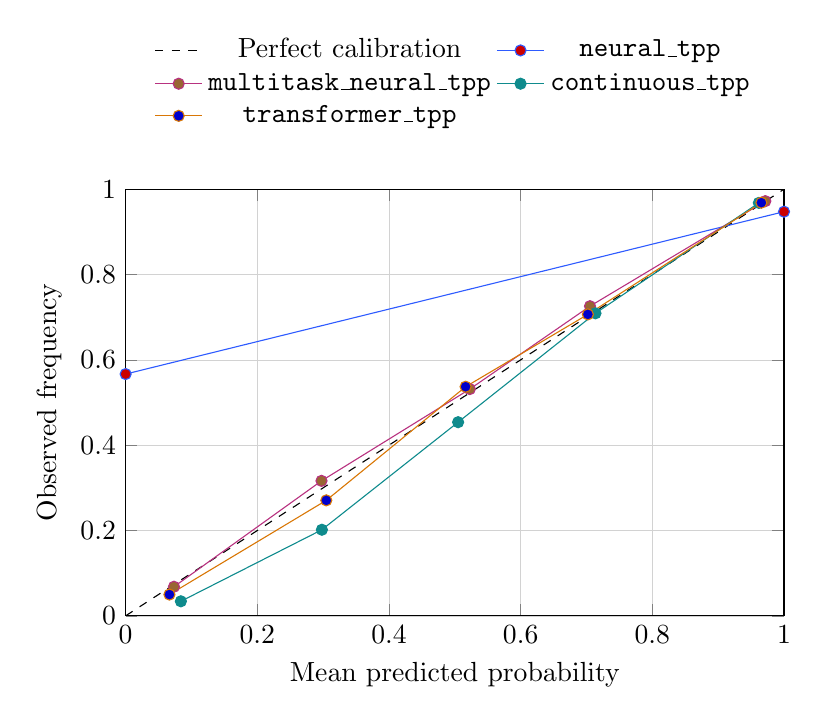
\begin{tikzpicture}
\begin{axis}[
  width=0.82\textwidth,
  height=7.0cm,
  xmin=0,
  xmax=1,
  ymin=0,
  ymax=1,
  xlabel={Mean predicted probability},
  ylabel={Observed frequency},
  legend style={at={(0.5,1.12)}, anchor=south, legend columns=2, draw=none},
  grid=both,
  grid style={line width=.1pt, draw=gray!20},
  major grid style={line width=.2pt, draw=gray!35},
]
\addplot[dashed, black] coordinates {(0,0) (1,1)};
\addplot+[color=neural, mark=*] coordinates {
  (0.0,0.5667) (1.0,0.9473)
};
\addplot+[color=multitask, mark=*] coordinates {
  (0.0734,0.0682) (0.2975,0.3164) (0.5228,0.5315) (0.7053,0.7258) (0.9716,0.9720)
};
\addplot+[color=continuous, mark=*] coordinates {
  (0.0839,0.0341) (0.2981,0.2018) (0.5050,0.4539) (0.7136,0.7091) (0.9618,0.9679)
};
\addplot+[color=transformer, mark=*] coordinates {
  (0.0665,0.0499) (0.3048,0.2707) (0.5164,0.5370) (0.7021,0.7066) (0.9656,0.9684)
};
\legend{Perfect calibration,\texttt{neural\_tpp},\texttt{multitask\_neural\_tpp},\texttt{continuous\_tpp},\texttt{transformer\_tpp}}
\end{axis}
\end{tikzpicture}
\caption{Pooled reliability curves for fixed-time condition forecasts on the adaptive \(60/20\) benchmark. Empty calibration bins are omitted. The direct-condition models lie much closer to the diagonal than the rollout-derived \texttt{neural\_tpp}, whose condition probabilities are concentrated near \(0\) and \(1\).}
\label{fig:calibration}
\end{figure}

\section{Evaluation}

The current benchmark evaluates:

\begin{enumerate}
  \item one-step next-event prediction
  \item short-horizon rollout forecasting
  \item fixed-time condition forecasting at \(10s\), \(30s\), and \(60s\)
\end{enumerate}

These three forecast tasks answer different questions.

\textbf{One-step next-event forecasting.}
This is the most local prediction task. At context index \(i\), the model is given the observed history \(\mathcal{H}_i\) and explicit state \(s_i\), and it must predict the very next discrete event:
\[
(\hat{m}_{i+1}, \hat{t}_{i+1}).
\]
The target is the immediate next realized event \((m_{i+1}, t_{i+1})\). This task measures whether the model understands the fine-grained event mechanics of the system: what kind of event fires next, and approximately when.

\textbf{Short-horizon rollout forecasting.}
This is an autoregressive sequence forecast rather than a single-step forecast. Starting from \((\mathcal{H}_i, s_i)\), the model predicts the next event, updates a replay state with that prediction, then predicts again from its own synthetic future. If the rollout horizon is \(K\), the predicted future is
\[
\hat{\mathcal{R}}_{i,K}
=
\{(\hat{m}_{i+1}, \hat{t}_{i+1}), \dots, (\hat{m}_{i+K}, \hat{t}_{i+K})\}.
\]
This forecast is compared with the realized \(K\)-event future
\[
\mathcal{R}_{i,K}
=
\{(m_{i+1}, t_{i+1}), \dots, (m_{i+K}, t_{i+K})\}.
\]
In the current benchmark, \(K \in \{5,10\}\). The rollout task is stricter than one-step prediction because errors compound. A model that is good at the first next event but poor at maintaining state consistency will degrade quickly under rollout.

\textbf{Fixed-time condition forecasting.}
This task asks a higher-level operational question: what traffic condition will hold after a fixed amount of time has passed? For horizon \(h \in \{10s,30s,60s\}\), the model predicts a vector of binary conditions
\[
\hat{\mathbf{c}}_{i,h}
=
(\hat{c}_{i,h,1}, \dots, \hat{c}_{i,h,K_c}),
\]
where each dimension corresponds to a named traffic condition. The target is obtained by advancing either the real event trace or a model rollout to time \(t_i + h\), reconstructing the future state \(s(t_i+h)\), and evaluating the condition flags on that state.

This task is different in meaning from event forecasting. It does not primarily ask whether the model gets each intervening arrival or departure exactly right. Instead, it asks whether the model correctly anticipates a more general future regime of the intersection.

The condition definitions used in the current benchmark are thresholded functions of replay-state queues:
\[
\mathrm{congested}(s) = \mathbf{1}\{Q_{\mathrm{tot}} \ge 12\},
\]
\[
\mathrm{severe\_queue}(s) = \mathbf{1}\{\max_{\ell} q_\ell \ge 6\},
\]
\[
\mathrm{ns\_pressure\_high}(s) = \mathbf{1}\{Q_{\mathrm{NS}} \ge 8\},
\qquad
\mathrm{ew\_pressure\_high}(s) = \mathbf{1}\{Q_{\mathrm{EW}} \ge 8\},
\]
\[
\mathrm{pressure\_imbalance}(s) = \mathbf{1}\{|Q_{\mathrm{NS}} - Q_{\mathrm{EW}}| \ge 5\}.
\]
These conditions should be interpreted as coarse traffic regimes rather than exact physical thresholds from a real deployment. They were chosen to create a meaningful distinction between light, moderate, and asymmetric demand states in the simulated environment.

The benchmark therefore spans three semantic levels:
\begin{itemize}
  \item event-level forecasting: what happens next
  \item sequence-level forecasting: what chain of events unfolds next
  \item state/condition-level forecasting: what regime the system will be in after some horizon
\end{itemize}
Each level is useful for a different downstream purpose. Event forecasts are closest to process modeling, rollout forecasts test stability under autoregressive use, and condition forecasts are closest to operational decision support.

The one-step event metrics are defined as follows. Let \(N\) be the number of evaluated prediction points.

The main event metrics are:
\begin{itemize}
  \item type accuracy
  \item family accuracy
  \item time MAE
  \item time RMSE
  \item within-2-seconds rate
\end{itemize}

Type accuracy measures exact event-label agreement:
\[
\mathrm{Acc}_{\mathrm{type}} =
\frac{1}{N}\sum_{i=1}^{N}\mathbf{1}\{\hat{m}_{i+1}=m_{i+1}\}.
\]
Family accuracy is coarser. If \(\mathrm{fam}(m)\) maps an event label to one of \{\texttt{phase\_change}, \texttt{vehicle\_arrival}, \texttt{vehicle\_departure}\}, then
\[
\mathrm{Acc}_{\mathrm{family}} =
\frac{1}{N}\sum_{i=1}^{N}
\mathbf{1}\{\mathrm{fam}(\hat{m}_{i+1})=\mathrm{fam}(m_{i+1})\}.
\]
This metric is useful when the model gets the event family right even if it misses the exact subtype.

Let the timing residual be
\[
\varepsilon_i = \hat{t}_{i+1} - t_{i+1}.
\]
Then the absolute timing metrics are
\[
\mathrm{MAE}_{t} = \frac{1}{N}\sum_{i=1}^{N} |\varepsilon_i|,
\qquad
\mathrm{RMSE}_{t} =
\sqrt{\frac{1}{N}\sum_{i=1}^{N} \varepsilon_i^2 }.
\]
The within-2-seconds rate is
\[
\mathrm{Hit@2s} =
\frac{1}{N}\sum_{i=1}^{N}\mathbf{1}\{|\varepsilon_i|\le 2\}.
\]
This last metric is operationally useful because many event forecasts can tolerate small timing error without changing the implied traffic interpretation.

The main condition metrics are:
\begin{itemize}
  \item balanced accuracy
  \item Brier score
  \item log loss
\end{itemize}

For a binary condition \(c \in \{0,1\}\), let \(\hat{y}_i \in \{0,1\}\) be the thresholded prediction and \(\hat{p}_i \in [0,1]\) the predicted probability. If \(\mathrm{TPR}\) and \(\mathrm{TNR}\) are the true positive rate and true negative rate, then balanced accuracy is
\[
\mathrm{BalAcc} = \frac{1}{2}(\mathrm{TPR}+\mathrm{TNR}).
\]
Balanced accuracy is preferred over raw accuracy because several traffic conditions, especially at longer horizons, are class-imbalanced and can otherwise be dominated by the majority class.

The Brier score measures squared probability error:
\[
\mathrm{Brier} = \frac{1}{N}\sum_{i=1}^{N}(\hat{p}_i-c_i)^2.
\]
Lower values indicate probabilities that are numerically close to the true outcomes.

The log loss is
\[
\mathrm{LogLoss} =
-\frac{1}{N}\sum_{i=1}^{N}
\left[
c_i \log \hat{p}_i + (1-c_i)\log(1-\hat{p}_i)
\right].
\]
This metric penalizes overconfident errors much more strongly than the Brier score, which makes it informative for decision-support use cases where poorly calibrated confidence is costly.

The benchmark also reports per-family and per-condition breakdowns. Those stratified views are important because a single pooled metric can hide qualitatively different behavior: a model may excel on departures but struggle on phase changes, or it may be well calibrated for congestion while remaining poorly calibrated for imbalance conditions.

Calibration is evaluated in two complementary ways. First, the benchmark reports Brier score and log loss, which summarize probabilistic quality numerically. Second, it computes pooled calibration bins over predicted condition probabilities. If a bin contains predictions in a score range \([u_j, u_{j+1})\), then the reported calibration point is
\[
\left(
\frac{1}{|B_j|}\sum_{i \in B_j}\hat{p}_i,
\frac{1}{|B_j|}\sum_{i \in B_j} c_i
\right).
\]
Plotting these points against the diagonal \(y=x\) yields a reliability curve. Curves near the diagonal indicate that predicted probabilities match observed frequencies, while curves above or below the diagonal indicate systematic underconfidence or overconfidence.

\section{Results}

\subsection{Primary Benchmark: Adaptive 60/20}

The strongest current benchmark is the larger adaptive run with:
\begin{itemize}
  \item \texttt{train-runs = 60}
  \item \texttt{eval-runs = 20}
\end{itemize}

Figure~\ref{fig:onestep} summarizes one-step results on this benchmark.

\begin{figure}[H]
\centering
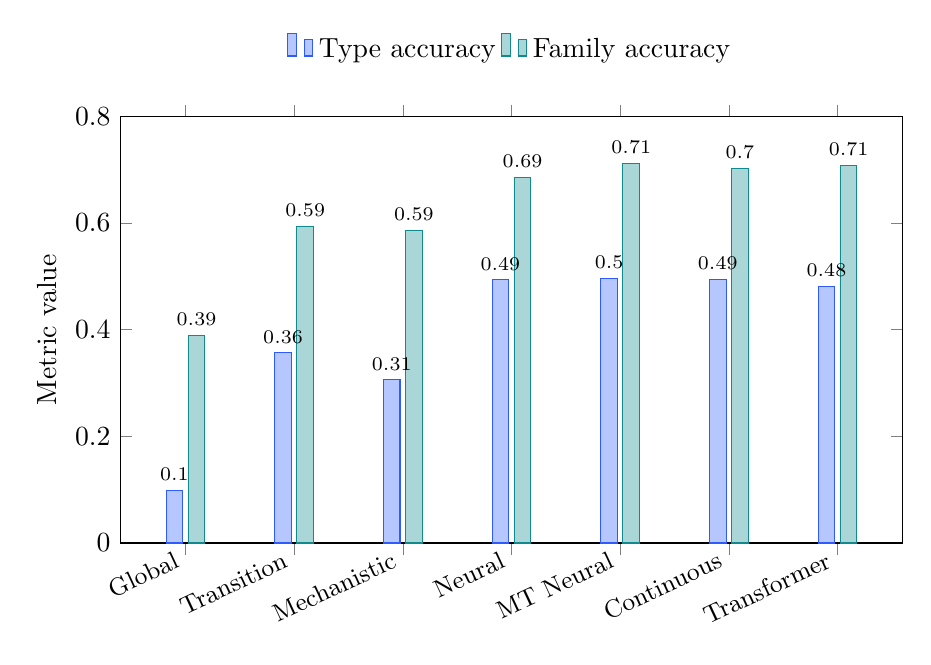
\begin{tikzpicture}
\begin{axis}[
  width=0.95\textwidth,
  height=7.0cm,
  ybar,
  bar width=6pt,
  ymin=0,
  ymax=0.80,
  enlarge x limits=0.10,
  symbolic x coords={Global,Transition,Mechanistic,Neural,MT Neural,Continuous,Transformer},
  xtick=data,
  xticklabel style={rotate=25, anchor=east, font=\small},
  legend style={at={(0.5,1.10)}, anchor=south, legend columns=2, draw=none},
  ylabel={Metric value},
  nodes near coords,
  nodes near coords style={font=\scriptsize, /pgf/number format/fixed, /pgf/number format/precision=2},
]
\addplot[fill=neural!35, draw=neural] coordinates {
  (Global,0.0986) (Transition,0.3567) (Mechanistic,0.3060) (Neural,0.4936) (MT Neural,0.4962) (Continuous,0.4941) (Transformer,0.4813)
};
\addplot[fill=continuous!35, draw=continuous] coordinates {
  (Global,0.3894) (Transition,0.5933) (Mechanistic,0.5865) (Neural,0.6852) (MT Neural,0.7125) (Continuous,0.7028) (Transformer,0.7083)
};
\legend{Type accuracy, Family accuracy}
\end{axis}
\end{tikzpicture}
\caption{One-step event accuracy metrics on the adaptive \(60/20\) benchmark. Only accuracy-valued metrics are combined in this figure. The strongest learned models are tightly clustered, with \texttt{multitask\_neural\_tpp} slightly ahead on exact and family-level event identification.}
\label{fig:onestep}
\end{figure}

\begin{figure}[H]
\centering
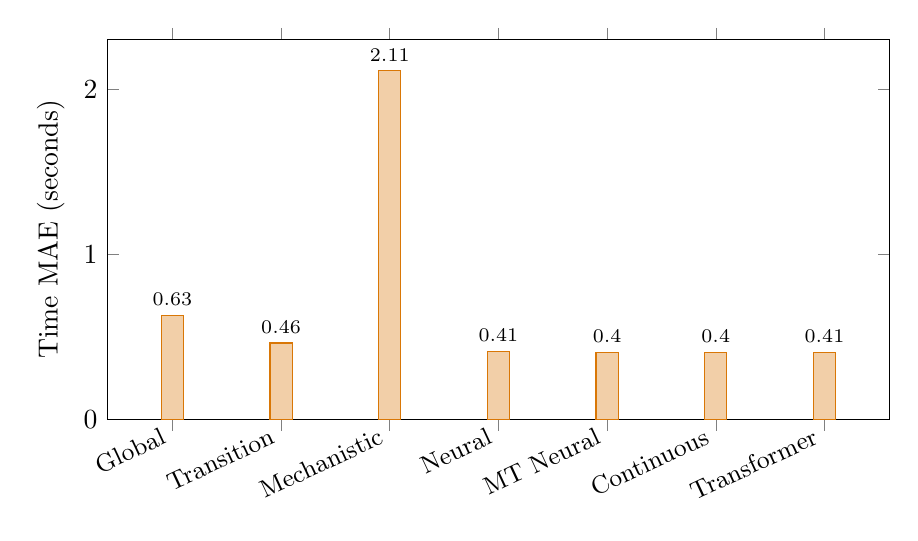
\begin{tikzpicture}
\begin{axis}[
  width=0.95\textwidth,
  height=6.4cm,
  ybar,
  bar width=8pt,
  ymin=0,
  ymax=2.30,
  enlarge x limits=0.10,
  symbolic x coords={Global,Transition,Mechanistic,Neural,MT Neural,Continuous,Transformer},
  xtick=data,
  xticklabel style={rotate=25, anchor=east, font=\small},
  ylabel={Time MAE (seconds)},
  nodes near coords,
  nodes near coords style={font=\scriptsize, /pgf/number format/fixed, /pgf/number format/precision=2},
]
\addplot[fill=transformer!35, draw=transformer] coordinates {
  (Global,0.6309) (Transition,0.4618) (Mechanistic,2.1114) (Neural,0.4087) (MT Neural,0.4049) (Continuous,0.4025) (Transformer,0.4054)
};
\end{axis}
\end{tikzpicture}
\caption{One-step timing error on the adaptive \(60/20\) benchmark. This figure is separated from the accuracy metrics because MAE is measured in seconds rather than normalized score units. \texttt{continuous\_tpp} is best on timing, with the other learned models close behind.}
\label{fig:onestep_time}
\end{figure}

The main one-step conclusions are:
\begin{itemize}
  \item \texttt{multitask\_neural\_tpp} has the best exact type accuracy: \(0.4962\)
  \item \texttt{multitask\_neural\_tpp} also has the best family accuracy: \(0.7125\)
  \item \texttt{continuous\_tpp} has the best time MAE: \(0.4025\)
\end{itemize}

\subsection{Fixed-Horizon Condition Forecasting}

Figure~\ref{fig:conditions} summarizes the fixed-horizon condition task on the same adaptive \(60/20\) benchmark.

\begin{figure}[H]
\centering
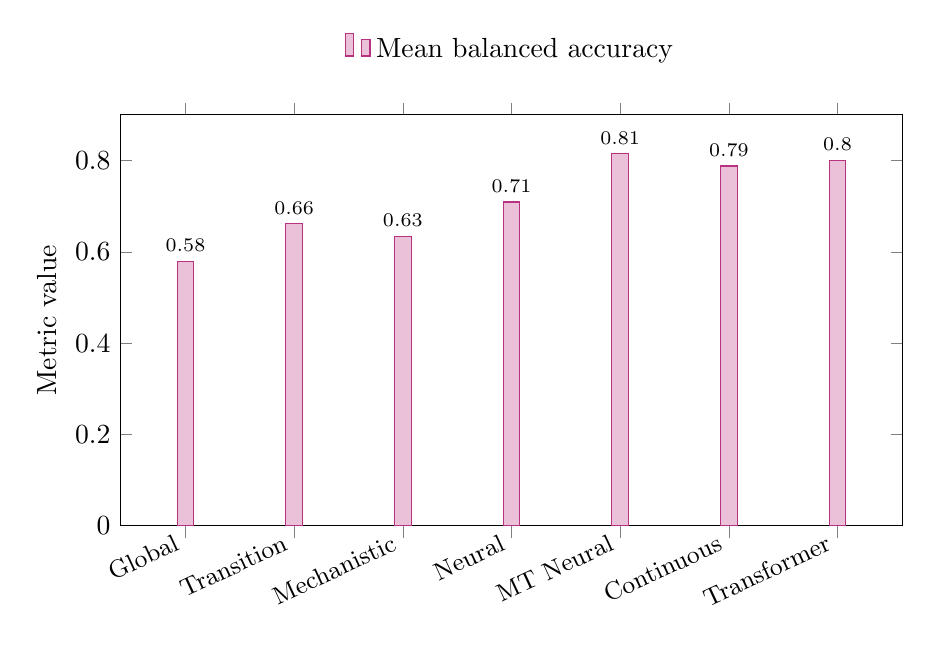
\begin{tikzpicture}
\begin{axis}[
  width=0.95\textwidth,
  height=6.8cm,
  ybar,
  bar width=6pt,
  ymin=0,
  ymax=0.90,
  enlarge x limits=0.10,
  symbolic x coords={Global,Transition,Mechanistic,Neural,MT Neural,Continuous,Transformer},
  xtick=data,
  xticklabel style={rotate=25, anchor=east, font=\small},
  legend style={at={(0.5,1.10)}, anchor=south, legend columns=1, draw=none},
  ylabel={Metric value},
  nodes near coords,
  nodes near coords style={font=\scriptsize, /pgf/number format/fixed, /pgf/number format/precision=2},
]
\addplot[fill=multitask!30, draw=multitask] coordinates {
  (Global,0.5790) (Transition,0.6613) (Mechanistic,0.6344) (Neural,0.7091) (MT Neural,0.8146) (Continuous,0.7880) (Transformer,0.8009)
};
\legend{Mean balanced accuracy}
\end{axis}
\end{tikzpicture}
\caption{Fixed-horizon condition balanced accuracy averaged across all condition definitions and horizons on the adaptive \(60/20\) benchmark. This plot contains only normalized accuracy-style values. The direct-condition models are clearly separated from the rollout-derived condition forecasts.}
\label{fig:conditions}
\end{figure}

\begin{figure}[H]
\centering
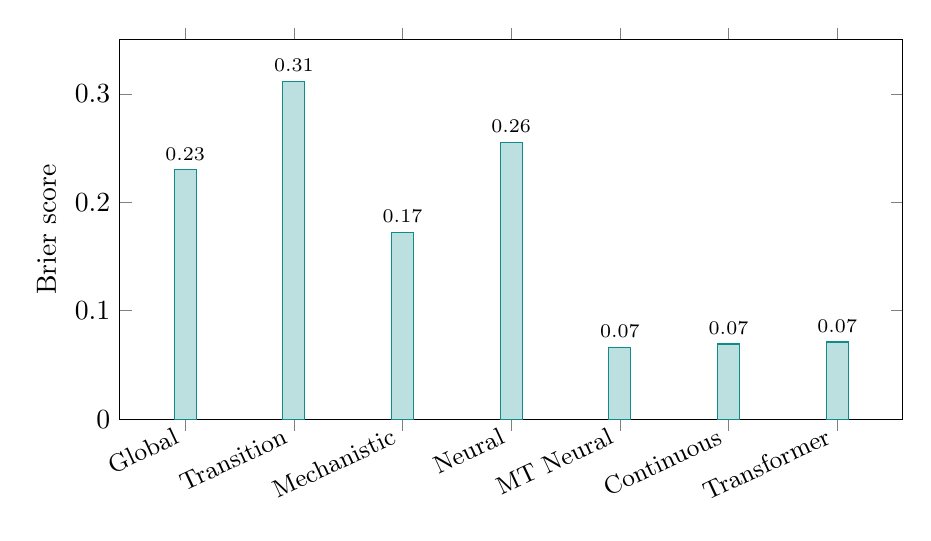
\begin{tikzpicture}
\begin{axis}[
  width=0.95\textwidth,
  height=6.4cm,
  ybar,
  bar width=8pt,
  ymin=0,
  ymax=0.35,
  enlarge x limits=0.10,
  symbolic x coords={Global,Transition,Mechanistic,Neural,MT Neural,Continuous,Transformer},
  xtick=data,
  xticklabel style={rotate=25, anchor=east, font=\small},
  ylabel={Brier score},
  nodes near coords,
  nodes near coords style={font=\scriptsize, /pgf/number format/fixed, /pgf/number format/precision=2},
]
\addplot[fill=continuous!28, draw=continuous] coordinates {
  (Global,0.2299) (Transition,0.3113) (Mechanistic,0.1724) (Neural,0.2550) (MT Neural,0.0659) (Continuous,0.0693) (Transformer,0.0712)
};
\end{axis}
\end{tikzpicture}
\caption{Fixed-horizon probabilistic quality measured by mean Brier score. Lower is better. \texttt{multitask\_neural\_tpp}, \texttt{continuous\_tpp}, and \texttt{transformer\_tpp} all produce much better calibrated condition probabilities than the rollout-derived baselines.}
\label{fig:brier}
\end{figure}

\begin{figure}[H]
\centering
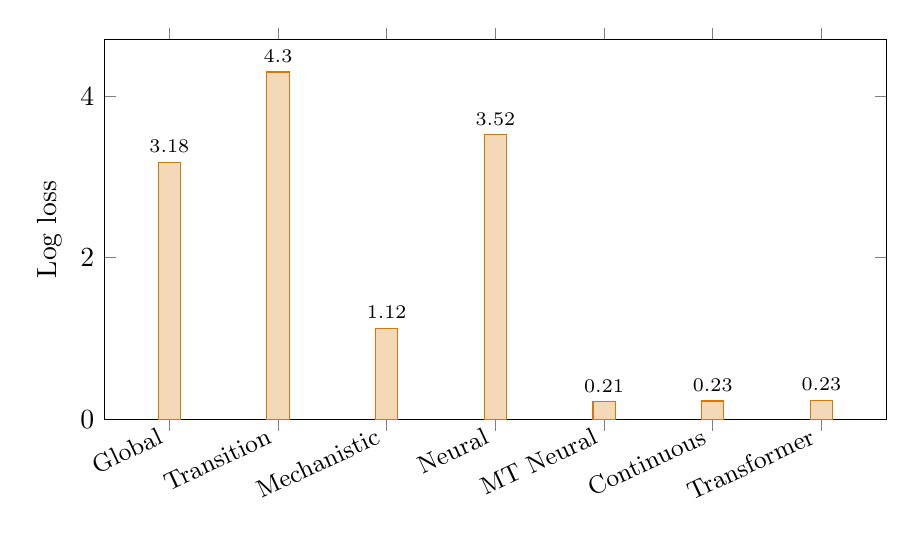
\begin{tikzpicture}
\begin{axis}[
  width=0.95\textwidth,
  height=6.4cm,
  ybar,
  bar width=8pt,
  ymin=0,
  ymax=4.7,
  enlarge x limits=0.10,
  symbolic x coords={Global,Transition,Mechanistic,Neural,MT Neural,Continuous,Transformer},
  xtick=data,
  xticklabel style={rotate=25, anchor=east, font=\small},
  ylabel={Log loss},
  nodes near coords,
  nodes near coords style={font=\scriptsize, /pgf/number format/fixed, /pgf/number format/precision=2},
]
\addplot[fill=transformer!28, draw=transformer] coordinates {
  (Global,3.1767) (Transition,4.3002) (Mechanistic,1.1229) (Neural,3.5223) (MT Neural,0.2136) (Continuous,0.2250) (Transformer,0.2311)
};
\end{axis}
\end{tikzpicture}
\caption{Fixed-horizon probabilistic quality measured by mean log loss. Lower is better. This view isolates overconfident errors and shows how strongly the direct-condition heads improve confidence quality.}
\label{fig:logloss}
\end{figure}

The most important result in the report is that direct-condition models are now decisively stronger on condition forecasting:

\begin{center}
\begin{tabular}{lccc}
\toprule
Model & Mean Balanced Accuracy & Mean Brier & Mean Log Loss \\
\midrule
\texttt{global\_rate} & 0.5790 & 0.2299 & 3.1767 \\
\texttt{transition} & 0.6613 & 0.3113 & 4.3002 \\
\texttt{mechanistic} & 0.6344 & 0.1724 & 1.1229 \\
\texttt{neural\_tpp} & 0.7091 & 0.2550 & 3.5223 \\
\texttt{multitask\_neural\_tpp} & \textbf{0.8146} & \textbf{0.0659} & \textbf{0.2136} \\
\texttt{continuous\_tpp} & 0.7880 & 0.0693 & 0.2250 \\
\texttt{transformer\_tpp} & 0.8009 & 0.0712 & 0.2311 \\
\bottomrule
\end{tabular}
\end{center}

\subsection{Baseline Simulator vs Richer Simulator at the Same Scale}

The repository now also includes a matched comparison between the earlier baseline-style simulator and the newer richer simulator, both under adaptive control and both at the same \(60/20\) benchmark scale. This comparison isolates the effect of changing the traffic environment itself rather than changing the train/eval budget or controller regime.

The richer simulator differs from the baseline simulator in three main ways:
\begin{itemize}
  \item arrivals are no longer stationary Poisson with a single fixed rate per lane; they include time-varying corridor pulses and bursty sub-platoons
  \item service is no longer governed by one shared saturation headway; headways now vary by lane
  \item turning-share penalties induce lane-specific discharge behavior, so not all queues clear equally quickly even when they have green
\end{itemize}

Figure~\ref{fig:baseline_richer_conditions} compares mean fixed-horizon condition balanced accuracy between the two simulator profiles. This figure uses only normalized balanced-accuracy values, so it stays on a single metric scale.

\begin{figure}[H]
\centering
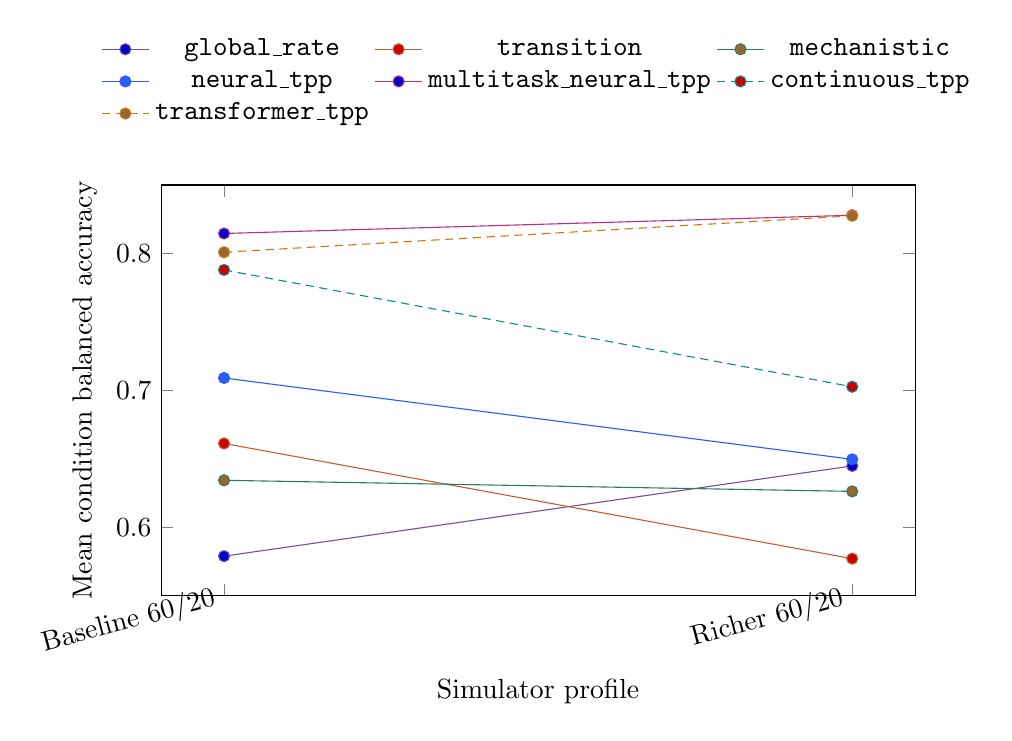
\begin{tikzpicture}
\begin{axis}[
  width=0.92\textwidth,
  height=6.8cm,
  ymin=0.55,
  ymax=0.85,
  xlabel={Simulator profile},
  ylabel={Mean condition balanced accuracy},
  symbolic x coords={Baseline 60/20, Richer 60/20},
  xtick=data,
  xticklabel style={rotate=15, anchor=east},
  legend style={at={(0.5,1.12)}, anchor=south, legend columns=3, draw=none},
  mark options={solid},
]
\addplot+[color=global, mark=*] coordinates {(Baseline 60/20,0.5790) (Richer 60/20,0.6449)};
\addplot+[color=transition, mark=*] coordinates {(Baseline 60/20,0.6613) (Richer 60/20,0.5772)};
\addplot+[color=mechanistic, mark=*] coordinates {(Baseline 60/20,0.6344) (Richer 60/20,0.6263)};
\addplot+[color=neural, mark=*] coordinates {(Baseline 60/20,0.7091) (Richer 60/20,0.6497)};
\addplot+[color=multitask, mark=*] coordinates {(Baseline 60/20,0.8146) (Richer 60/20,0.8279)};
\addplot+[color=continuous, mark=*] coordinates {(Baseline 60/20,0.7880) (Richer 60/20,0.7027)};
\addplot+[color=transformer, mark=*] coordinates {(Baseline 60/20,0.8009) (Richer 60/20,0.8275)};
\legend{\texttt{global\_rate}, \texttt{transition}, \texttt{mechanistic}, \texttt{neural\_tpp}, \texttt{multitask\_neural\_tpp}, \texttt{continuous\_tpp}, \texttt{transformer\_tpp}}
\end{axis}
\end{tikzpicture}
\caption{Mean fixed-time condition balanced accuracy under the earlier baseline simulator and the richer simulator, both at adaptive \(60/20\) scale. The richer simulator still makes exact event prediction harder, but after the latest direct-condition refinements it now exposes a stronger separation between the best calibrated condition models and the weaker empirical baselines.}
\label{fig:baseline_richer_conditions}
\end{figure}

Table~\ref{tab:baseline_richer_event} complements that condition-level view with one-step event metrics for representative models. Each cell reports \(\texttt{baseline} / \texttt{richer}\) at the same adaptive \(60/20\) scale.

\begin{table}[H]
\centering
\small
\begin{tabular}{lcccc}
\toprule
Metric & Transition & MT Neural & Continuous & Transformer \\
\midrule
Type accuracy & 0.357 / 0.259 & 0.496 / 0.441 & 0.494 / 0.429 & 0.481 / 0.426 \\
Family accuracy & 0.593 / 0.491 & 0.713 / 0.682 & 0.703 / 0.693 & 0.708 / 0.648 \\
Time MAE & 0.462 / 0.472 & 0.405 / 0.403 & 0.403 / 0.402 & 0.405 / 0.411 \\
Mean cond. bal. acc. & 0.661 / 0.577 & 0.815 / 0.828 & 0.788 / 0.703 & 0.801 / 0.828 \\
\bottomrule
\end{tabular}
\caption{Representative one-step and condition-summary results under the earlier baseline simulator and the richer simulator, both at adaptive \(60/20\) scale. Each cell is reported on a single metric scale and uses the same train/eval budget.}
\label{tab:baseline_richer_event}
\end{table}

This baseline-versus-richer comparison changes the interpretation of the benchmark in an important way. The earlier simulator was still useful, but it was more regular: arrivals were simpler, effective service was more homogeneous, and the queue dynamics were easier to summarize with a small set of empirical averages. The richer simulator breaks that regularity. Under the richer profile, type accuracy falls for nearly every learned model, which indicates that exact event identity has become genuinely harder to infer from local history alone. At the same time, timing MAE changes very little for the strongest learned models, especially \texttt{continuous\_tpp} and \texttt{multitask\_neural\_tpp}. That is a good sign: the richer simulator is not merely injecting arbitrary noise, but specifically making the mark-prediction problem more heterogeneous while leaving the temporal-scale modeling problem largely intact.

The condition metrics become more informative in the richer environment, but the most important update is that the latest direct-condition refinements now hold up under that harder setting. \texttt{continuous\_tpp} still drops from \(0.7880\) to \(0.7027\), which confirms that richer heterogeneity exposes real weaknesses in that model's condition path. By contrast, the stronger direct-condition specialists now remain at or above their baseline-simulator condition scores: \texttt{multitask\_neural\_tpp} rises from \(0.8146\) to \(0.8279\), and the improved \texttt{transformer\_tpp} rises from \(0.8009\) to \(0.8275\). That does not mean the richer simulator is easier overall; exact event typing still gets harder. Rather, it means the richer benchmark now rewards models that can fuse longer event context with explicit state-aware condition structure.

At the same time, the richer simulator sharpens the distinction between model families. The empirical \texttt{transition} baseline degrades strongly on both exact event prediction and condition balanced accuracy, which indicates that first-order transition statistics are no longer sufficient once arrivals become bursty and lane service becomes heterogeneous. The \texttt{mechanistic} baseline behaves differently: its exact type prediction degrades substantially, but its probabilistic condition metrics improve and its pressure-imbalance behavior becomes more structured. This is consistent with a hand-built queue model that still captures coarse directional pressure, but is less able to match the exact fine-grained event stream once lane-specific service rules matter more.

A final focused transformer pass further refined that story. Lowering the transformer's condition-loss weight from \(0.10\) to \(0.08\) preserved its richer-simulator condition advantage while recovering family accuracy in a focused rerun, reaching family accuracy \(0.6759\) with mean condition balanced accuracy \(0.8285\). That result is not yet folded into the all-model richer comparison table above, but it reinforces the same conclusion: on the richer simulator, the transformer is no longer a distant third condition model. It is effectively tied with \texttt{multitask\_neural\_tpp} when its condition path and loss balance are tuned to the task.

\subsection{Fixed vs Adaptive at the Same Scale}

The repository now includes a matching fixed-control benchmark at the same \(60/20\) scale, so the regime comparison can be made without mixing dataset sizes. Figure~\ref{fig:regime60} compares mean fixed-time condition balanced accuracy under fixed and adaptive control only, which keeps the comparison on a single metric scale and a single train/eval configuration.

\begin{figure}[H]
\centering
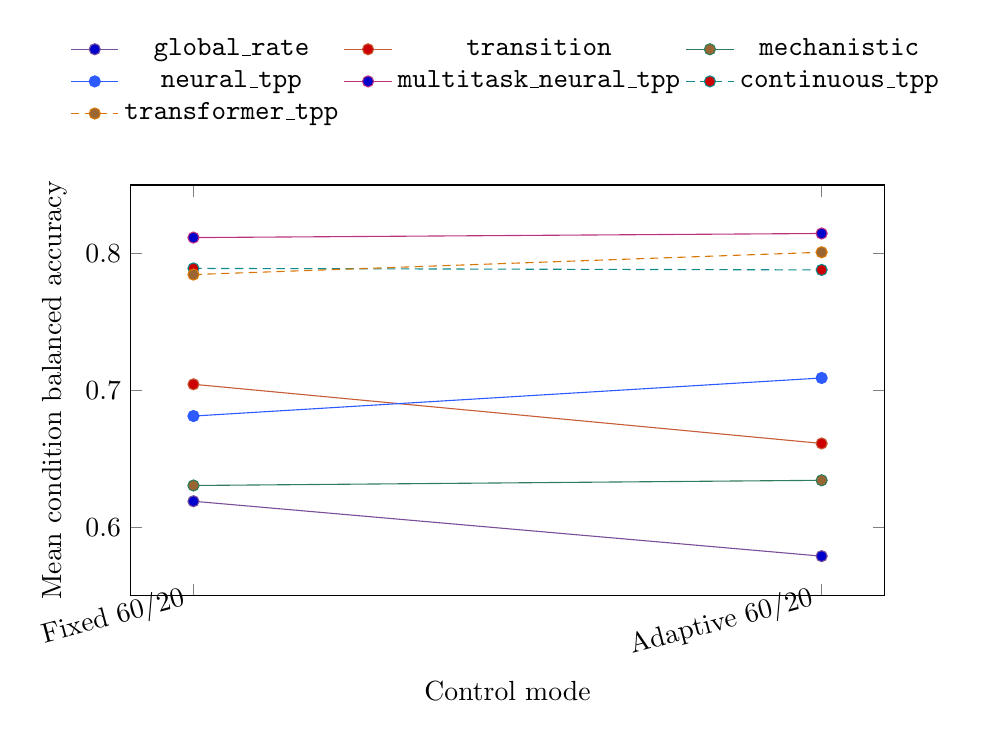
\begin{tikzpicture}
\begin{axis}[
  width=0.92\textwidth,
  height=6.8cm,
  ymin=0.55,
  ymax=0.85,
  xlabel={Control mode},
  ylabel={Mean condition balanced accuracy},
  symbolic x coords={Fixed 60/20, Adaptive 60/20},
  xtick=data,
  xticklabel style={rotate=15, anchor=east},
  legend style={at={(0.5,1.12)}, anchor=south, legend columns=3, draw=none},
  mark options={solid},
]
\addplot+[color=global, mark=*] coordinates {(Fixed 60/20,0.6191) (Adaptive 60/20,0.5790)};
\addplot+[color=transition, mark=*] coordinates {(Fixed 60/20,0.7045) (Adaptive 60/20,0.6613)};
\addplot+[color=mechanistic, mark=*] coordinates {(Fixed 60/20,0.6306) (Adaptive 60/20,0.6344)};
\addplot+[color=neural, mark=*] coordinates {(Fixed 60/20,0.6813) (Adaptive 60/20,0.7091)};
\addplot+[color=multitask, mark=*] coordinates {(Fixed 60/20,0.8116) (Adaptive 60/20,0.8146)};
\addplot+[color=continuous, mark=*] coordinates {(Fixed 60/20,0.7891) (Adaptive 60/20,0.7880)};
\addplot+[color=transformer, mark=*] coordinates {(Fixed 60/20,0.7846) (Adaptive 60/20,0.8009)};
\legend{\texttt{global\_rate}, \texttt{transition}, \texttt{mechanistic}, \texttt{neural\_tpp}, \texttt{multitask\_neural\_tpp}, \texttt{continuous\_tpp}, \texttt{transformer\_tpp}}
\end{axis}
\end{tikzpicture}
\caption{Mean fixed-time condition balanced accuracy under fixed and adaptive control for the same \(60/20\) benchmark scale. The strongest direct-condition models are robust across regimes, while the mechanistic baseline benefits much more strongly from the simpler fixed controller.}
\label{fig:regime60}
\end{figure}

The regime comparison yields three useful conclusions. First, the direct-condition learned models are robust: \texttt{multitask\_neural\_tpp} remains the strongest condition forecaster in both settings, with mean balanced accuracy \(0.8116\) under fixed control and \(0.8146\) under adaptive control. Second, \texttt{continuous\_tpp} is nearly regime-invariant on the same metric (\(0.7891\) fixed versus \(0.7880\) adaptive), which suggests its timing-aware inductive bias transfers cleanly across controller behavior. Third, \texttt{mechanistic} changes much more sharply with regime: its one-step time MAE improves from \(2.1114\) under adaptive control to \(0.6006\) under fixed control, which confirms that hand-structured controller assumptions help most when the controller itself is simpler and more regular.

Table~\ref{tab:per-condition-regime} makes the regime comparison more specific by breaking mean condition balanced accuracy out by condition class for representative models. Each cell reports \(\texttt{fixed} / \texttt{adaptive}\) at the same \(60/20\) benchmark scale.

\begin{table}[H]
\centering
\small
\begin{tabular}{lcccc}
\toprule
Condition & Mechanistic & MT Neural & Continuous & Transformer \\
\midrule
Congested & 0.722 / 0.742 & 0.764 / 0.782 & 0.703 / 0.752 & 0.754 / 0.800 \\
Severe queue & 0.707 / 0.738 & 0.806 / 0.806 & 0.795 / 0.730 & 0.768 / 0.798 \\
NS pressure & 0.589 / 0.584 & 0.873 / 0.870 & 0.871 / 0.879 & 0.852 / 0.812 \\
EW pressure & 0.577 / 0.603 & 0.834 / 0.870 & 0.816 / 0.857 & 0.799 / 0.858 \\
Imbalance & 0.557 / 0.504 & 0.780 / 0.745 & 0.761 / 0.723 & 0.750 / 0.738 \\
\bottomrule
\end{tabular}
\caption{Per-condition mean balanced accuracy under fixed and adaptive control for representative models at the same \(60/20\) scale. Each cell shows fixed/adaptive performance, not a mixed-scale aggregate.}
\label{tab:per-condition-regime}
\end{table}

This per-condition view shows that the regime effect is not uniform. Adaptive control helps the learned models most on coarse congestion and east-west pressure conditions, where controller responsiveness changes the future queue regime. Fixed control remains relatively favorable for imbalance-oriented forecasts, especially for the mechanistic model, because the simpler controller makes directional pressure asymmetries more regular and easier to anticipate from hand-crafted logic.

\section{Interpretation}

Three patterns matter most:

\begin{enumerate}
  \item \textbf{Event prediction and condition prediction are now clearly different tasks.}
  Strong next-event models are not automatically strong condition forecasters.

  \item \textbf{Direct condition heads are worth the complexity.}
  They are now clearly better than deriving conditions only from autoregressive event rollout.

  \item \textbf{The strongest models win for understandable architectural reasons.}
  Their inductive biases line up with the actual structure of the benchmark.
\end{enumerate}

The strongest model in the report for condition forecasting is \texttt{multitask\_neural\_tpp}. It works well for three reasons. First, its shared recurrent encoder is strong enough to summarize the local event process, so it does not lose the sequential information needed to understand whether the system is building toward arrivals, departures, or a phase transition. Second, it does not stop at next-event prediction: it has direct heads trained specifically for the \(10s\), \(30s\), and \(60s\) condition tasks. That means the representation is optimized for the exact forecasting question being asked in evaluation. Third, the model uses calibrated probability outputs, so its good balanced accuracy is matched by genuinely strong Brier and log-loss values rather than only favorable thresholded decisions.

\texttt{continuous\_tpp} works especially well on timing because its hidden state evolves as a function of elapsed time, not just event count. That matters in this simulator because arrivals and departures are irregularly spaced, and queue state can change meaningfully as time passes even if no new event has yet been observed. The continuous-time decay gives the model a more natural way to represent asynchronous event gaps, which is why it remains the best one-step timing model while also staying competitive on condition forecasts once direct condition heads are added.

\texttt{transformer\_tpp} works well for a different reason: it can directly re-attend to multiple earlier events rather than compressing everything into a purely recurrent state. In this application, the next condition is often determined by a pattern across several recent arrivals, departures, and phase changes, not only by the last one or two events. The transformer therefore benefits from broader context access, especially when queue pressure is building over several alternating events. Earlier in the project it lagged the best multitask GRU clearly, but the richer benchmark changed that. Once its condition path was separated from the event trunk and the condition-loss balance was tuned more carefully, it became effectively tied with \texttt{multitask\_neural\_tpp} on richer condition forecasting while remaining competitive on event prediction.

\texttt{neural\_tpp} without direct condition heads is an instructive contrast. It is a good next-event model, but a weaker condition model, because it must answer condition questions indirectly by rolling out its own predicted future events. Any small event-level errors then accumulate before the final condition is computed. This explains why it can look respectable on one-step event metrics while remaining much worse on Brier score and log loss for condition forecasts.

Condition calibration is therefore not a cosmetic addition to the benchmark. It changes the interpretation of what a ``good'' forecast means. A high balanced accuracy model that is badly calibrated may still be risky in downstream use, because its confidence scores cannot be trusted. By contrast, the strongest direct-condition models in this repository are not only more accurate after thresholding; they are also much better calibrated. That is why they improve simultaneously on balanced accuracy, Brier score, and log loss. The practical meaning is that they are better not only at deciding whether a condition will happen, but also at expressing how certain they are about that decision.

\texttt{mechanistic} performs better than the simplest empirical baselines because it explicitly encodes queue and controller structure. It knows that departures depend on service availability and that phase changes follow a constrained controller policy. That structural prior helps it remain competitive on some condition-style quantities even though it lacks the flexibility of the learned direct-condition models. Its weakness is that it cannot adapt as well to the full stochastic variability present in the simulator, especially when the effective future depends on subtle combinations of arrival bursts and state history.

The new fixed-versus-adaptive \(60/20\) comparison makes the model behavior more interpretable. Under fixed control, \texttt{mechanistic} becomes much more effective because its structural assumptions are closer to the true generator. Under adaptive control, those same assumptions become less reliable, and the learned models gain relative advantage. This is exactly the kind of pattern one would hope to see in a credible benchmark: hand-crafted structure helps when the environment is structurally aligned with it, while learned models become more valuable as controller behavior becomes more state-dependent.

The new baseline-versus-richer comparison adds a second important robustness check. It shows that the current ranking is not purely an artifact of one very simple environment. The richer simulator changes the leaderboard quantitatively without collapsing it qualitatively: the weaker empirical models degrade more sharply, \texttt{continuous\_tpp} loses headroom on condition forecasting, and the two strongest direct-condition models --- \texttt{multitask\_neural\_tpp} and \texttt{transformer\_tpp} --- emerge as the most robust richer-simulator specialists. That is exactly the kind of pattern one would hope to see if the richer simulator is increasing structural difficulty rather than merely rescaling all results uniformly.

\section{Limitations and Next Steps}

Important limitations remain:
\begin{itemize}
  \item only one application domain is implemented
  \item the simulator is still intentionally simple
  \item the learned models are supervised predictors rather than full likelihood-based temporal point processes
\end{itemize}

The strongest next step is:
\begin{enumerate}
  \item deepen the same-scale fixed-versus-adaptive comparison with per-condition calibration analysis
  \item continue improving the strongest direct-condition models before adding another new architecture family
  \item continue expanding the richer simulator with turning movements, spillback-style constraints, and less stationary demand regimes
\end{enumerate}

\section{Conclusion}

The repository now supports a substantially more credible benchmark than the initial version. The main conclusions are:

\begin{itemize}
  \item the traffic simulator is now a useful testbed for both event and condition forecasting
  \item direct-condition heads are a major improvement over event-rollout-derived condition forecasts
  \item larger train/eval sets materially improved result quality
  \item \texttt{multitask\_neural\_tpp} remains the strongest overall condition forecaster in the main benchmark tables, but \texttt{transformer\_tpp} is now effectively tied with it on the richer adaptive benchmark after the latest condition-path refinement
  \item \texttt{continuous\_tpp} remains strongest on timing
  \item \texttt{transformer\_tpp} improved enough to become a top-tier richer-simulator condition model rather than merely a secondary contender
  \item \texttt{mechanistic} is far more competitive under fixed control than adaptive control, which validates the regime sensitivity of the benchmark
  \item the richer simulator makes event forecasting materially harder while preserving the main qualitative advantage of direct-condition learned models
\end{itemize}

\end{document}
